%%
%% This is file `sample-sigconf-authordraft.tex',
%% generated with the docstrip utility.
%%
%% The original source files were:
%%
%% samples.dtx  (with options: `all,proceedings,bibtex,authordraft')
%% 
%% IMPORTANT NOTICE:
%% 
%% For the copyright see the source file.
%% 
%% Any modified versions of this file must be renamed
%% with new filenames distinct from sample-sigconf-authordraft.tex.
%% 
%% For distribution of the original source see the terms
%% for copying and modification in the file samples.dtx.
%% 
%% This generated file may be distributed as long as the
%% original source files, as listed above, are part of the
%% same distribution. (The sources need not necessarily be
%% in the same archive or directory.)
%%
%%
%% Commands for TeXCount
%TC:macro \cite [option:text,text]
%TC:macro \citep [option:text,text]
%TC:macro \citet [option:text,text]
%TC:envir table 0 1
%TC:envir table* 0 1
%TC:envir tabular [ignore] word
%TC:envir displaymath 0 word
%TC:envir math 0 word
%TC:envir comment 0 0
%%
%%
%% The first command in your LaTeX source must be the \documentclass
%% command.
%%
%% For submission and review of your manuscript please change the
%% command to \documentclass[manuscript, screen, review]{acmart}.
%%
%% When submitting camera ready or to TAPS, please change the command
%% to \documentclass[sigconf]{acmart} or whichever template is required
%% for your publication.
%%
%%
\documentclass[sigconf,authordraft]{acmart}

%%
%% \BibTeX command to typeset BibTeX logo in the docs
\AtBeginDocument{%
  \providecommand\BibTeX{{%
    Bib\TeX}}}

%% Rights management information.  This information is sent to you
%% when you complete the rights form.  These commands have SAMPLE
%% values in them; it is your responsibility as an author to replace
%% the commands and values with those provided to you when you
%% complete the rights form.
\setcopyright{acmlicensed}
\copyrightyear{2018}
\acmYear{2018}
\acmDOI{XXXXXXX.XXXXXXX}

%% These commands are for a PROCEEDINGS abstract or paper.
\acmConference[Conference acronym 'XX]{Make sure to enter the correct
  conference title from your rights confirmation emai}{June 03--05,
  2018}{Woodstock, NY}
%%
%%  Uncomment \acmBooktitle if the title of the proceedings is different
%%  from ``Proceedings of ...''!
%%
%%\acmBooktitle{Woodstock '18: ACM Symposium on Neural Gaze Detection,
%%  June 03--05, 2018, Woodstock, NY}
\acmISBN{978-1-4503-XXXX-X/18/06}


%%
%% Submission ID.
%% Use this when submitting an article to a sponsored event. You'll
%% receive a unique submission ID from the organizers
%% of the event, and this ID should be used as the parameter to this command.
%%\acmSubmissionID{123-A56-BU3}

%%
%% For managing citations, it is recommended to use bibliography
%% files in BibTeX format.
%%
%% You can then either use BibTeX with the ACM-Reference-Format style,
%% or BibLaTeX with the acmnumeric or acmauthoryear sytles, that include
%% support for advanced citation of software artefact from the
%% biblatex-software package, also separately available on CTAN.
%%
%% Look at the sample-*-biblatex.tex files for templates showcasing
%% the biblatex styles.
%%

%%
%% The majority of ACM publications use numbered citations and
%% references.  The command \citestyle{authoryear} switches to the
%% "author year" style.
%%
%% If you are preparing content for an event
%% sponsored by ACM SIGGRAPH, you must use the "author year" style of
%% citations and references.
%% Uncommenting
%% the next command will enable that style.
%%\citestyle{acmauthoryear}


%%
%% end of the preamble, start of the body of the document source.
\begin{document}

%%
%% The "title" command has an optional parameter,
%% allowing the author to define a "short title" to be used in page headers.
\title{Using LLM for code generation and repair in functional programming assessments: challenges and potential
}

%%
%% The "author" command and its associated commands are used to define
%% the authors and their affiliations.
%% Of note is the shared affiliation of the first two authors, and the
%% "authornote" and "authornotemark" commands
%% used to denote shared contribution to the research.
% \author{Ben Trovato}
% \authornote{Both authors contributed equally to this research.}
% \email{trovato@corporation.com}
% \orcid{1234-5678-9012}
% \author{G.K.M. Tobin}
% \authornotemark[1]
% \email{webmaster@marysville-ohio.com}
% \affiliation{%
%   \institution{Institute for Clarity in Documentation}
%   \city{Dublin}
%   \state{Ohio}
%   \country{USA}
% }


%%
%% By default, the full list of authors will be used in the page
%% headers. Often, this list is too long, and will overlap
%% other information printed in the page headers. This command allows
%% the author to define a more concise list
%% of authors' names for this purpose.
\renewcommand{\shortauthors}{Trovato et al.}

%%
%% The abstract is a short summary of the work to be presented in the
%% article.
\begin{abstract}

% While there already exists a line of work evaluating the performance of LLMs such as ChatGPT in solving independent programming tasks, few of them investigate how the model could behave in solving programming assignments/homework that is designed to fit students' learning trajectories. 

The recent introduction of ChatGPT has drawn significant attention
from both industry and academia due to its impressive capabilities in
solving a diverse range of tasks, including language translation, text
summarization, and computer programming.
% Unlike previous large language models, ChatGPT effectively bridges
% the gap between human and AI performance in multiple key domains. 
Its capability for writing, modifying, and even
correcting code together with its ease of use and access is already 
dramatically impacting computer science education. 
%To comprehensively evaluate such impact, it is essential to assess
%its ability to solve programming tasks in the context of computer
%science education. 
This paper aims to explore how well ChatGPT can perform in an
introductory-level functional language programming course.  Our comprehensive evaluation provides valuable
insights into ChatGPT's impact from both student and instructor
perspectives. Additionally, we identify several potential benefits
that ChatGPT can offer to both groups. Overall, we believe that this
study significantly clarifies and advances our understanding of
ChatGPT's capabilities and potential impact on computer science education.
\end{abstract}

%%
%% The code below is generated by the tool at http://dl.acm.org/ccs.cfm.
%% Please copy and paste the code instead of the example below.
%%
% \begin{CCSXML}
% <ccs2012>
%  <concept>
%   <concept_id>00000000.0000000.0000000</concept_id>
%   <concept_desc>Do Not Use This Code, Generate the Correct Terms for Your Paper</concept_desc>
%   <concept_significance>500</concept_significance>
%  </concept>
%  <concept>
%   <concept_id>00000000.00000000.00000000</concept_id>
%   <concept_desc>Do Not Use This Code, Generate the Correct Terms for Your Paper</concept_desc>
%   <concept_significance>300</concept_significance>
%  </concept>
%  <concept>
%   <concept_id>00000000.00000000.00000000</concept_id>
%   <concept_desc>Do Not Use This Code, Generate the Correct Terms for Your Paper</concept_desc>
%   <concept_significance>100</concept_significance>
%  </concept>
%  <concept>
%   <concept_id>00000000.00000000.00000000</concept_id>
%   <concept_desc>Do Not Use This Code, Generate the Correct Terms for Your Paper</concept_desc>
%   <concept_significance>100</concept_significance>
%  </concept>
% </ccs2012>
% \end{CCSXML}

\ccsdesc[500]{Do Not Use This Code~Generate the Correct Terms for Your Paper}
\ccsdesc[300]{Do Not Use This Code~Generate the Correct Terms for Your Paper}
\ccsdesc{Do Not Use This Code~Generate the Correct Terms for Your Paper}
\ccsdesc[100]{Do Not Use This Code~Generate the Correct Terms for Your Paper}

%%
%% Keywords. The author(s) should pick words that accurately describe
%% the work being presented. Separate the keywords with commas.
% \keywords{Do, Not, Us, This, Code, Put, the, Correct, Terms, for,
%   Your, Paper}
%% A "teaser" image appears between the author and affiliation
%% information and the body of the document, and typically spans the
%% page.
% \begin{teaserfigure}
%   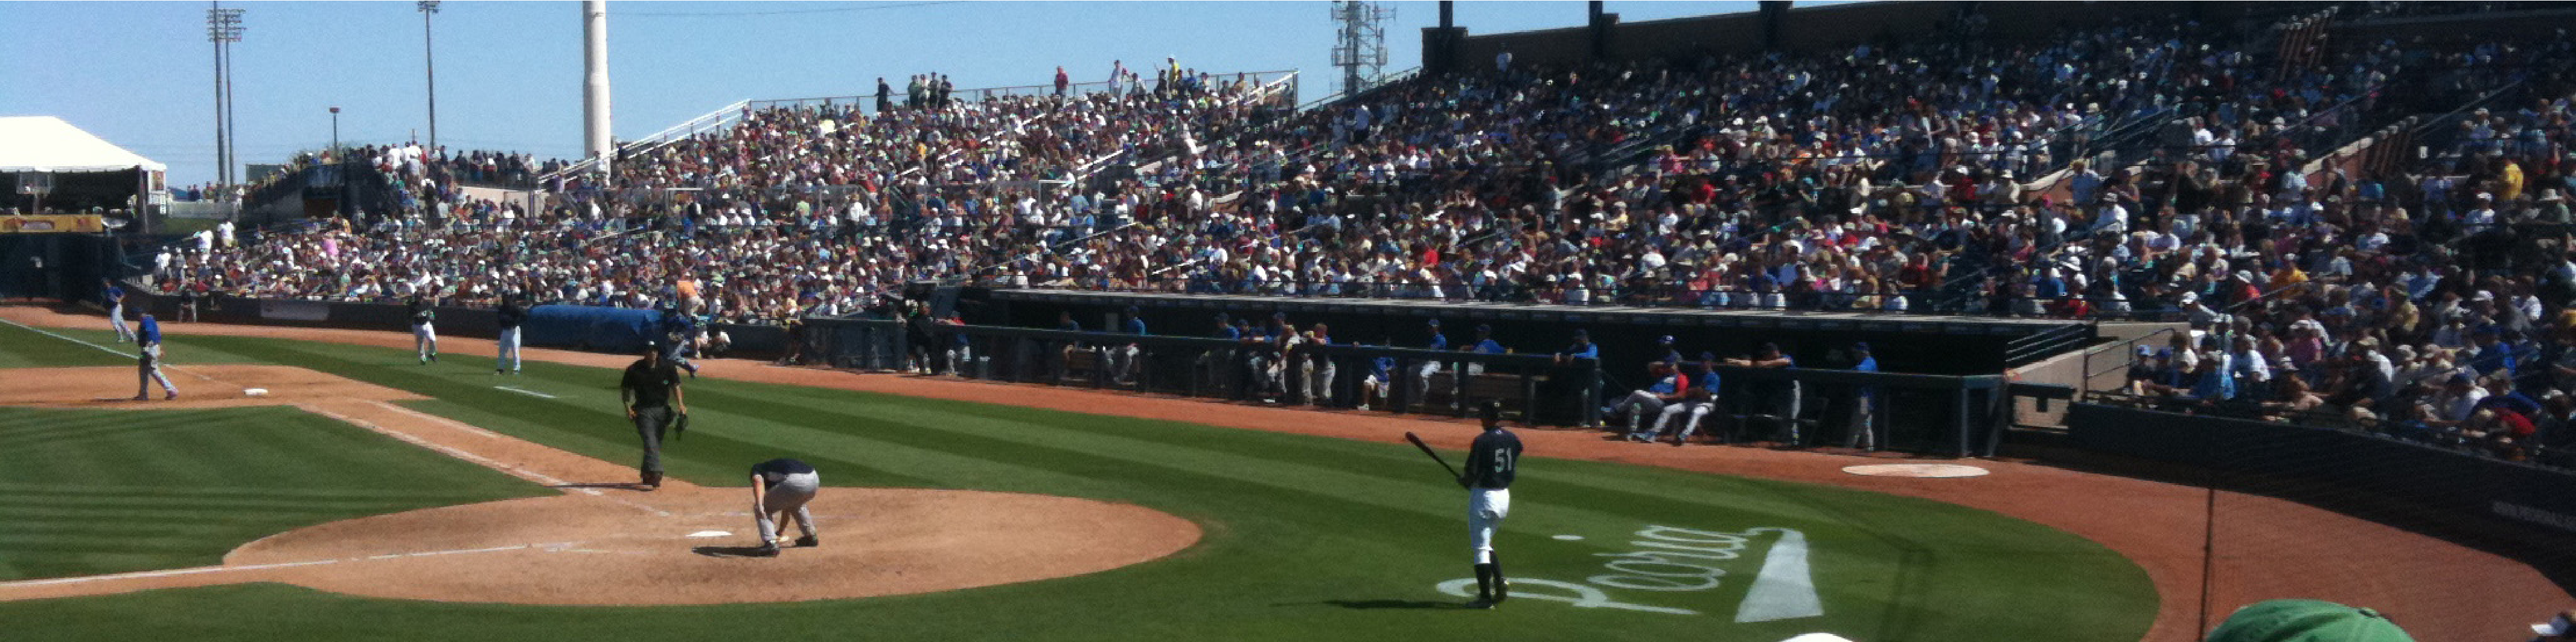
\includegraphics[width=\textwidth]{sampleteaser}
%   \caption{Seattle Mariners at Spring Training, 2010.}
%   \Description{Enjoying the baseball game from the third-base
%   seats. Ichiro Suzuki preparing to bat.}
%   \label{fig:teaser}
% \end{teaserfigure}

\received{20 February 2007}
\received[revised]{12 March 2009}
\received[accepted]{5 June 2009}

%%
%% This command processes the author and affiliation and title
%% information and builds the first part of the formatted document.
\maketitle

\section{Introduction}

Large Language Models (LLMs) have made significant strides in various domains, including natural language processing, machine translation, and text summarization. Among these applications, the use of LLMs for program synthesis and generation has been particularly noteworthy. Projects such as OpenAI's Codex and DeepMind's AlphaCode have demonstrated the impressive ability of LLMs to generate code, showcasing their potential in automating programming tasks.


Recently, LLMs have been evaluated in introductory programming courses that utilize languages like Java and Python. These studies have shown that LLMs can effectively generate programs, assisting students in writing and understanding code. However, the application of LLMs in the context of statically typed functional programming languages, such as OCaml, remains relatively unexplored.

In this study, we evaluate ChatGPT's performance in an introductory functional language programming course that focuses on OCaml based on all homework assignments and exams from the 2022 fall semester.
Our goal is to assess the grade that ChatGPT would receive on each assessment and overall in the course. To compare the model's performance to actual students enrolled in the course, we also rank its performance with respect to actual grade distributions in the course. 


The objective of this research is to evaluate the effectiveness of LLMs in teaching statically typed functional programming. Specifically, we aim to investigate whether LLMs can autonomously solve programming assignments and tasks in OCaml. While previous research has focused on dynamically typed languages like Python and statically typed object-oriented languages like Java, there is a lack of studies on statically typed functional programming languages.

Furthermore, we seek to understand if LLMs can repair code and provide useful feedback to students. This capability could position LLMs as valuable teaching assistants, offering immediate feedback on syntax, type, and logical errors in students' code. Exploring this potential aligns with broader educational goals, such as enhancing student learning experiences and providing additional support in programming courses.

Understanding the capabilities of different LLMs in writing and fixing code is crucial for several reasons. It allows us to assess whether one LLM is more powerful than another—a question that has been studied for Python and Java but not for statically typed functional programming languages . Additionally, insights into how students can effectively use LLMs in a course can help instructors design programming exercises that promote academic integrity and prevent misuse of LLMs for cheating.

Evaluating LLMs poses several challenges. We often lack knowledge about their training data, raising questions about the reproducibility of results. Additionally, the variability in LLM outputs can lead to inconsistent results, complicating the evaluation process. Moreover, equity and inclusion concerns arise, as the cost of evaluating LLMs may be prohibitive for some reviewers or instructors.

Despite these challenges, our research aims to shed light on the practical and conceptual aspects of using LLMs for programming education, particularly in statically typed functional programming languages. By addressing these questions, we hope to contribute to the growing body of knowledge on LLMs and their potential to transform programming education.

\section{Background(related work?)}

% The development of language models has been a gradual process that has spanned several decades. Early efforts to develop computer systems capable of understanding natural language date back to the 1950s and 1960s, with researchers such as Joseph Weizenbaum and Alan Turing making significant contributions in the field of natural language processing (NLP).

% \allen{Here we combine the original back and related work together.}

In recent years, the development of large language models has accelerated with the advances in computing hardware such as GPU and TPU and the availability of vast amounts of training data. The success of these large language models is largely due to the transition in deep learning architecture from RNN (recurrent neural network) \cite{RNN} to Transformer models \cite{Transformer}. In fact, most successful large language models today such as BERT (Bidirectional Encoder Representations from Transformers) \cite{BERT} and the T5 (Text-to-Text Transfer Transformer) \cite{T5} are based on the Transformer. %Over the years, there has been a clear trend of large language models growing in size, accompanied by an increase in their capabilities. 

% One of the most notable examples of this trend is the GPT (Generative Pre-trained Transformer) family of models developed by OpenAI. The first GPT model, GPT-1 \cite{GPT}, was released in 2018 and had 117 million parameters. This was followed by GPT-2 \cite{GPT-2} in 2019, which had 1.5 billion parameters and generated significant media attention due to its impressive language generation capabilities. GPT-3 \cite{GPT-3}, released in 2020, had a staggering 175 billion parameters and was described as a "breakthrough" in the field of natural language processing. 

One of the most notable examples of this trend is the GPT (Generative Pre-trained Transformer) family of models developed by OpenAI. Early language models like GPT-1 \cite{GPT} had a relatively small number of parameters, but with the introduction of GPT-2 \cite{GPT-2} and GPT-3 \cite{GPT-3}, the size of language models has grown substantially. GPT-3, for instance, has 175 billion parameters, making it one of the largest language models to date. On the other hand, ChatGPT, an enhanced version of OpenAI's GPT-3, also referred to as GPT-3.5, has proven to outperform GPT-3 in almost every benchmark. With these large language models, we have seen significant improvements in natural language processing (NLP) tasks such as text generation, summarization, and translation. Additionally, the growing capabilities of large language models have enabled them to be used for various applications, including chatbots, virtual assistants, and even code generation. As the capabilities of these models continue to expand, we can expect to see further advancements in NLP and other areas of AI. 

The increasing popularity of large language models such as ChatGPT is due to their ability to enable users to  interact with them via only natural language texts. Such ability is deeply linked to their capability of predicting the next word given prior words in a sentence. Since most natural language-related tasks can be framed as the next-word prediction, ChatGPT as well as other GPT models are expected to perform various tasks if they are well-engineered as prompts/instructions. Thus, it is well-expected that ChatGPT could perform differently when different prompt engineering techniques are used to guide its responses. With the right prompt engineering, ChatGPT can be used to perform a wide range of tasks, such as language translation, summarization, and even code generation. As a result, ChatGPT has the potential to become a valuable tool in various domains, from education to healthcare, as it can help users complete tasks and solve problems using only natural language inputs.

When it comes to the impact of ChatGPT on computer science education, it is worth noting that the model's ability to understand and generate code represents a significant improvement over previous models. This breakthrough makes ChatGPT a tool that will transform computer science education.
% It has the potential to  by providing a powerful platform for learning and teaching programming concepts. 
As we have seen from previous work \cite{chen2021codex}, ChatGPT's predecessors
are capable of understanding and generating code in commonly-used programming languages such as Python, Java, and C. Thus, in this study, we focus on evaluating and analyzing ChatGPT's performance in understanding concepts and generating code in OCaml - a functional programming language, in a real university course teaching environment. Subsequently, based on our empirical results, we aim to investigate how both students and instructors/TAs can benefit from ChatGPT. While there are potential merits to using ChatGPT in computer science education, we also discuss its limitations and potential risks.


\subsection{Overview of The Course}
Our study concerns students in a second-year undergraduate computer science course at X\footnote{The name is intentionally anonymized for the double-blind review.} university. The course introduces concepts about functional programming and programming paradigms. It is offered every semester with more than 300 registered undergraduate students. In this study, we use assignments and exam questions from Fall 2022, since ChatGPT is trained on data before 2021, so it is less likely that the model has seen those questions before.

The course has ten weekly programming assignments each worth 3\%, a midterm exam worth 20\%, and a final exam worth 50\%   of the total grade. Table \ref{overview} presents a brief overview of the course content and related homework assignments. Each homework consists of several programming tasks to implement functions and test cases. All homework assignments were hosted on Learn-OCaml, an online programming platform for OCaml that allows students to edit, compile, test, and debug code all in one place. We used a modified version of Learn-OCaml \cite{10.1145/3341719} by Hameer and Pientka with additional features such as style checking and evaluation of test cases written by students.




\section{Method}


% eval method
To evaluate how effectively LLMs can fix errors, we conducted experiments using various LLMs in different scenarios: zero-shot and one-shot. In the zero-shot scenario, we provided the LLM with a faulty program and asked it to generate a corrected version without any prior examples. In the one-shot scenario, we first provided the LLM with a faulty program and its corrected version. Then, we presented another similar faulty program and asked the LLM to generate the corrected version.

We identified similar programs by selecting faulty programs from a student's timeline, considering submissions either earlier or later in the course. This approach helped us evaluate the LLMs' ability to generalize error correction across different contexts.

For syntax errors, we randomly sampled 500 programs from student submissions, equally distributed among ten homework assignments (HW1-10) from Fall 2022. We used two modes for this evaluation: Mode A, where the prompt explicitly mentioned that the program contained a syntax error, and Mode B, where the prompt did not specify the type of error. We compared the results from Fall 2022 to those from Winter 2023 to validate the LLMs' performance.

For type errors, we followed a similar approach, sampling 500 programs from Fall 2022 and comparing them with Winter 2023 submissions. Additionally, we identified "hard stuck states" with the help of an expert, Jerry, to assess the LLMs' ability to resolve more challenging type errors.

For logical errors, we again sampled 500 programs from Fall 2022 and compared them with Winter 2023 submissions. This evaluation helped us understand how well LLMs could address more complex and nuanced errors in student code.

We also evaluated the LLMs' capability to write complete programs by providing them with 100 different programming assignments and assessing their performance. We measured the pass rate as the percentage of assignments where the LLM generated a correct solution that passed all tests on the first try. Additionally, we evaluated the success rate over multiple attempts (k = 1, 5, 10), recording the maximum grade achieved across these attempts.

We used two different modes for this evaluation: no feedback, where the LLM generated solutions without any intermediate feedback, and compiler feedback, where the LLM received one round of feedback from a compiler, allowing it to refine its solution before the final evaluation. For each program generated by the LLM, we recorded the highest score achieved over the three attempts. This comprehensive evaluation helped us understand the LLMs' potential in generating correct and high-quality code.

By conducting these evaluations, we aimed to gain insights into the strengths and limitations of different LLMs in both error correction and program generation tasks, particularly in the context of teaching statically typed functional programming languages like OCaml.
\section{Evaluation}

\section{Threats To Validity}
In our evaluation, we assume that the LLMs are already fully trained and that no additional re-training or learning occurs during the evaluation process. This assumption is crucial because it impacts the validity and reproducibility of our results. If any form of additional learning were to take place during the evaluation, it could skew the outcomes and lead to an overestimation of the LLMs' capabilities.

Furthermore, the variability in LLM outputs poses a challenge to the consistency of our findings. Since LLMs can produce different results given the same input on different occasions, this variability must be accounted for in our analysis. We mitigate this by averaging results over multiple runs, but inherent unpredictability remains a concern.

Another threat to validation arises from the unknown nature of the training data used to develop the LLMs. Without detailed knowledge of the datasets and the specific programming tasks the LLMs were exposed to during training, it is difficult to ascertain whether the models have been inadvertently trained on similar tasks or even specific examples present in our evaluation dataset. This could result in biased performance metrics that do not accurately reflect the models' generalization capabilities.

Additionally, the evaluation process itself could introduce biases. For example, the selection of faulty programs and the criteria for what constitutes a "similar" program may affect the outcomes. We have attempted to mitigate this by using a random sampling approach and defining clear criteria for similarity, but subjective decisions are unavoidable.

The cost and accessibility of running extensive evaluations with LLMs also present equity and inclusion concerns. Not all researchers or educators may have the resources to replicate our study, which could limit the generalizability and applicability of our findings across different contexts.


\section{Citations}

\section{Appendices}

If your work needs an appendix, add it before the
``\verb|\end{document}|'' command at the conclusion of your source
document.

Start the appendix with the ``\verb|appendix|'' command:
\begin{verbatim}
  \appendix
\end{verbatim}
and note that in the appendix, sections are lettered, not
numbered. This document has two appendices, demonstrating the section
and subsection identification method.


%%
%% The next two lines define the bibliography style to be used, and
%% the bibliography file.
\bibliographystyle{ACM-Reference-Format}
\bibliography{sample-base}


%%
%% If your work has an appendix, this is the place to put it.
\appendix

\section{Research Methods}


\end{document}
\endinput
%%
%% End of file `sample-sigconf-authordraft.tex'.
